% ------ headers globales y begin ---------------
\documentclass[11pt, a4paper, twoside]{article}
\usepackage{header_tp1}

\begin{document}{}
% -----------------------------------------------

\subsubsection{Descripción} 

desea contratar a un experto
por $D$ días consecutivos
para que éste pueda detectar si algún camión de la

El inspector \texttt{Rick A. Lapazta}, legendario\footnote{La leyenda dice que
junto a su compañero Zepas A. Poraki, son invictos en no hacer muy bien su
trabajo} empleado un puesto de control de camiones, es encomendado por la diosa
Mor\texttt{fea} durante un revelador sueño a la tarea de investigar si la
empresa \textit{il Raviolin} está transportando \texttt{sustancias ilegales}.
Luego de meses de investigación, y de arriesgar su pasiva e inspeccionista vida
intrusionando en el archivo secreto de la empresa descubre que realmente cuenta
con muy poca información: dispone de una lista en la anotó los datos importantes
de cada camión, la cantidad de antenas de cada uno de ellos, y el día en que
atravesarán el control. El inspector deduce posteriormente que la mayor o menor
cantidad de antenas de un camión no debe ser un factor influyente al momento de
transportar este tipo de sustancias, y que la mejor solución a sus problemas es
contratar a un \textit{experto}. 

Como dispone de una cantidad acotada de dinero, y sabe que el tercerizado le
cobrará una cantidad fija de dinero por cada día de trabajo el inspector busca,
dado un rango de días de inspección, maximizar la cantidad de camiones
inspeccionados, es decir que la mayor cantidad de camiones tienen que estar
pasando por el puesto durante el período de contración del experto. El inspector
conoce los días en que cada uno de los $n$ camiones de la empresa estará
pasando, pero desgraciadamente esta información puede o no estar dada en orden
cronológico, nadie lo sabe. El inspector olvidó mencionarlo, pero el experto es
de otro país, el reino de muy muy lejano, y la legislación de turismo de la zona
es muy dura, por lo que este sólo dispone de permiso realizar un viaje al puesto
de inspección.

El problema encomienda encontrar una solución al dilema del inspector, en donde
recibiendo como \textbf{datos de entrada} la cantidad de días ($D$), la cantidad
de camiones ($n$) y los días en que estos llegarán ($d_1$,$d_2$,...,$d_n$) se
deberá idear un algoritmo que lo resuelva con una complejidad
\textbf{estrictamente mejor que} \bigO{n^{2}}, siendo $n$ la cantidad total de
camiones. El resultado que se deberá obtener es el día inicial $d_i$ en que
convendría contratar al experto, y el total $c$ de camiones que serán
inspeccionados por el mismo.

Formato de entrada:
\[
  D\ n\ d1\ d2\ ...\ dn\
\]

Formato de salida:
\[
  d_i\ c
\]

\vspace{3em}

Si se contrata al experto por $D=3$ días consecutivos y en total hay $n=20$
camiones sospechosos ($c1,c2,...,c20$) que pasan por el puesto según se muestra
a continuación:

\begin{ejemplo}\hspace{0em}

  \begin{quote}
    \begin{verbatim}
    Entrada:
    3 20 10 10 9 4 1 1 1 1 1 2 6 6 6 4 5 5 5 5 5 9
    \end{verbatim}
  \end{quote}

    \begin{center}
      \begin{tabular}{|l|l|l|l|l|l|l|l|l|l|l|}
      	\hline
      	Día          &  $1$  & $2$   & $3$   & $4$   & $5$   & $6$ & $7$ & $8$ & $9$   & $10$  \\
      	\hline
      	Camiones     &  $c5$ & $c10$ & $c14$ & $c4$  & $c15$ & $c11$ &   &     & $c3$  & $c1$  \\
      				 &  $c6$ &       &       &       & $c16$ & $c12$ &   &     & $c20$ & $c2$  \\    
      				 &	$c7$ &       &       &       & $c17$ & $c13$ &   &     &       &       \\  
      				 &	$c8$ &       &       &       & $c18$ &       &   &     &       &       \\
      				 &	$c9$ &       &       &       & $c19$ &       &   &     &       &       \\
      	\hline
      \end{tabular}
    \end{center}

    El primer día del período de contratación será $d=4$ y habrán sido
  inspeccionados, durante los días \texttt{Día4}, \texttt{Día5} y \texttt{Día6},
  un total de $c=9$ camiones. 

  \begin{quote}
  \begin{verbatim}
  Salida:
  4 9
  \end{verbatim}
  \end{quote}

\end{ejemplo}

\begin{ejemplo}\hspace{0em}

  \begin{quote}
    \begin{verbatim}
    Entrada:
    3 20 1 2 7 1 1 1 1 1 1 1 7 7 7 1 4 4 4 4 4 7
    \end{verbatim}
  \end{quote}

  \begin{center}
    \begin{tabular}{|l|l|l|l|l|l|l|l|}
    	\hline
    	Día          &  $1$  & $2$   & $3$   & $4$    & $5$ & $6$ & $7$   \\
    	\hline
    	Camiones     &  $c5$ &       &       & $c15$  &     &     & $c11$ \\
    				 &  $c6$ &       &       & $c16$  &     &     & $c12$ \\    
    				 &	$c7$ &       &       & $c17$  &     &     & $c13$ \\  
    				 &	$c8$ &       &       & $c18$  &     &     & $c3$  \\
    				 &	$c9$ &       &       & $c19$  &     &     & $c20$ \\
    				 &	$c10$&       &       &        &     &     &       \\
    				 &	$c14$&       &       &        &     &     &       \\
    				 &	$c4$ &       &       &        &     &     &       \\
    				 &	$c1$ &       &       &        &     &     &       \\
    				 &	$c2$ &       &       &        &     &     &       \\
    	\hline
    \end{tabular}
  \end{center}

  Para este caso, el primer día del período de contratación será $d=1$ y habrán
  sido inspeccionados, durante los días \texttt{Día1}, \texttt{Día2} y
  \texttt{Día3}, un total de $c=10$ camiones.

  \begin{quote}
    \begin{verbatim}
    Salida:
    1 10
    \end{verbatim}
  \end{quote}

\end{ejemplo}

\subsubsection{Hipótesis de resolución}

Nos interesa saber cuál es el mejor día entre $d_1$ y $d_n$ para contratar al
experto. Desde el día elegido hasta el día $D - 1$, buscamos que la cantidad de
camiones sea máxima. Primero, entonces, ordenamos en forma creciente el conjunto
{$d_1$,...,$d_n$} dado. Sabemos que la solución pertenece a este conjunto.
Tenemos a $P(x)$ como la suma de la cantidad de camiones que pasan desde el día
$x$ hasta el día $x+D-1$. Nuestro algoritmo itera sobre cada elemento $d_i$ del
conjunto calculando P($d_i$), y guardando el elemento $e$ con P($e$) máximo
encontrado hasta el momento. Al final de las iteraciones, tenemos guardado el
elemento $e$ con P($e$) máximo en todo el conjunto. Devolvemos $e$ y P($e$).


\subsubsection{Justificación formal de correctitud}

Consideremos los días de llegada ordenados en forma creciente: $d_1 \le d_2 \le
\dots \le d_n$ son enteros \underline{positivos} al igual que $D$. \\ Definimos
P(x), donde $x \in \mathbb{N}$, como $\sum_{i=1}^{n} I(d_i)_{[x,x+D-1]}$. \\
Buscamos $d$ tal que $(\forall x)$ P(x) $\le$ P(d). \\ Veamos que $d \le d_n$:
\\ P$(d_n)=1$ pues $d_n \in [d_n,d_n + D - 1]$ pero $\forall x > d_n$, P(x)$=0$
pues $d_i < x, \forall i \in 1...n$.\\ Luego, si $d > d_n, d$ no es óptimo. \\
Veamos que existe un $d$ óptimo tal que $d=d_i$ para algún $i \in 1...n$. \\ Sea
$d'$ óptimo. \\ Sea $d=min_{i \in 1...n}$ $d_i \big| d_i \ge d'$. \\ P(d)$\ge$
P(d') pues $\forall i$ tal que $d_i \in [d',d'+D-1], d_i \in [d,d+D-1]$ ya que
$\nexists$ $j$ tal que $d' \le d_j < d$ y pues $d'+D-1 \le d+D-1$. \\ Luego,
hemos reducido el espacio de solución a $\{$ $d_1,...,d_n$$\}$.


\subsubsection{Cota de complejidad temporal}\label{sec:ej1cotatemporal}
El algoritmo utilizado es el siguiente:

\begin{algorithm}[H]
\caption{Algoritmo Camiones Sospechosos}\label{camionessospechosos}
\footnotesize\begin{algorithmic}[1]
	\Require
		\Statex $intervaloInspector \gets$ \Call{dameIntervaloInspector}{} \Comment{$integer$}
		\Statex $cantidadDeCamiones \gets$ \Call{dameCantidadCamiones}{} \Comment{$integer$}
		\Statex $fechasCamiones \gets$ \Call{dameFechasCamiones}{} \Comment{$arreglo\langle integer \rangle$}
	\Ensure
		\Statex \Call{Fecha Óptima Inspector}{} \Comment{$integer$}
		\Statex \Call{Cantidad De Camiones Analizados}{} \Comment{$integer$}
	\Statex
	
  \State \Call{ordenar}{fechasCamiones} \Comment{\bigO{n.\log n}}
  \State $inicioInter \gets 0$ \Comment{\bigO{1}}
  \State $finInter \gets 0$ \Comment{\bigO{1}}
  \State $mDia \gets 0$ \Comment{\bigO{1}}
  \State $mCantidadCamiones \gets 0$ \Comment{\bigO{1}}

  \While {$finInter < cantidadDeCamiones$} \Comment{ \texttt{Como máximo n interaciones}}
    \While {$ \Call{DiferenciaMenorAInterInspector}{inicioInter, finInter} $}
      \State $ finInter \gets finInter+1$
    \EndWhile 
  \If {$\Call{CantCamionesEn}{inicioInter, finInterl} < mCantidadCamiones$} \Comment{\bigO{1}}
    \State $ mDia \gets inicioInter$ \Comment{\bigO{1}}
    \State $ mCantidadCamiones \gets \Call{CantCamionesEn}{inicioInter,finInter}$ \Comment{\bigO{1}}
  \EndIf {}
  \State $inicioInter \gets inicioInter +1$
  \EndWhile \Comment{\texttt{ciclo} \bigO{n}}
  \State \Return {$mDia, mCantCamiones$}
  \State


	\Function{CantCamionesEn}{$inicioInter, finInter$}
  \State \Return { $finInter - inicioInter$ } \Comment{\bigO{1}}
	\EndFunction \Comment{\texttt{final} \bigO{1}}
  \State

	\Function{DiferenciaMenorAInterInspector}{$inicioInter, finInter$}
    \State $diferencia \gets fechasCamiones_{finInter} - fechasCamiones_{inicioInter}$ \Comment{\bigO{1}}
    \State \Return {$ finInter < cantidadDeCamiones \texttt{ and } diferencia < intervaloInspector $} \Comment{\bigO{1}}
	\EndFunction \Comment{\texttt{final} \bigO{1}}

	\Statex{}
\end{algorithmic}
\end{algorithm}


Consideremos la complejidad del ciclo for. A lo largo del ciclo se van
actualizando izq y der, y se va guardando el maximo que lleva  en si O(1).
¿Cuántas veces se actualizan izq y der? Pues, como van en forma creciente de 1 a
n, exactamente n veces cada una. El ciclo for tiene complejidad O(2n) = O(n). La
complejidad del algoritmo es finalmente O(n log n).

Como se puede ver el algorítmo tiene 2 partes bien diferenciadas: Primero tiene
un ordenamiento de un arreglo unidimensional. Para eso se usa el algorítmo de
ordenamiento que brinda a librería standard de \textit{c++}. En la documentación
de la misma se puede apreciar que su complejidad en el peor caso es de \bigO{n.
\log n}\footnote{http://www.cplusplus.com/reference/algorithm/sort/} donde
\textit{n} es la distancia que hay entre el primer y el último elemento que se
quieren ordenar. En este caso se necesita ordenar todo el arreglo, por lo que
termina siendo \bigO{n.\log n} con respecto al tamaño de la entrada.

Luego hay un bucle while. El bucle \texttt{mientras} se repite mientras que el
fin del intervalo a analizar se encuentre dentro del arreglo de camiones.

Apenas se entra al ciclo \texttt{mientras} hay otro ciclo, el cuál tiene una
complejidad de peor caso de \bigO{n}. Este ciclo interno se encarga de hacer
avanzar el puntero \textit{finInter} hasta que la diferencia entre de las fechas
entre el principio del intervalo a analizar y el final del intervalo a analizar
sea menor a \textit{intervaloInspector}. El peor caso posible en este ciclo
sería que la diferencia entre el la fecha mas próxima y la fecha mas lejana sea
menor a intervalo inspector. En ese caso sale del bucle porque se pasó del
máximo. Sim embargo si eso ocurre también se deja de cumplir la condición de la
guarda externa, por lo tanto el bucle externo también termina.


Es decir, ambas guardas dependen de la misma comparación entre \textit{finInter}
y \textit{cantCamiones}, por lo tanto cuando termine una va a terminar la otra.
Por otra parte \textit{finInter} siempre avanza. No hay ningún caso en el cuál
retroceda. Esto significa que siempre va a recorrer exactamente
\textit{cantCamiones}, es decir que en el peor de los casos va a haber
\texttt{n} iteraciones del ciclo. Como el resto de las operaciones son todas
\bigO{1} podemos concluir que el ciclo completo tiene una complejidad de
\bigO{n}


De esta manera el algorítmo termina teniendo una complejidad de \bigO{n.\log n +
n} = \bigO{n. \log n}. De esta manera la complejidad es estrictamente menor que
$\bigO{n^{2}}$.








\subsubsection{Verificación mediante casos de prueba}

A continuación presentamos distintas instancias que sirven para verificar que el programa funciona correctamente. \\ 
\\
Input: [D n $d_1$...$d_n$], Output: [d c] \\
\\
D: cant. de días de contratación del experto \\
n: cant.  total de camiones que pasan por el puesto \\
$d_i$ con $1 \le i \le n$: días de llegada de los camiones \\
d: día inicial del período de contratación del experto \\
c: cant. de camiones inspeccionados por el experto \\  
\\
Sea $L$ el intervalo de días en que llegan los camiones. \\
$L$ $=$ (máx $d_i$ $-$ mín $d_i$ $+ 1$) con $1 \le i \le n$. \\

De los datos de entrada y salida sabemos que: 

\begin{itemize}
    \item $1$ $\le$ D, n, $d_i$ (con $1$ $\le$ i $\le$ n).
	\item $1 \le $ c $\le$ n 
	\item $1 \le $ mín $d_i$ $\le$ d $\le$ máx $d_i$ 
\end{itemize}

Entonces, podemos separar el conjunto de soluciones en los siguientes casos: \\

\begin{tabular}{|l|l|l|l|}
	\hline
	Caso &  Condición  						              & Ej.Input      & Ej.Output \\
	\hline
	$1$  &  D$=$L, d$=$mín $d_i$, c$=$n    				  & 3 3 1 2 3     & 1 3 \\	
	$2$  &	D$>$L, d$=$mín $d_i$, c$=$n     		      & 5 3 1 2 3     & 1 3 \\
	\hline	
	$3$  &	D$<$L, d$=$mín $d_i$, c$<$n     			  & 3 4 1 2 5 1   & 1 3 \\
	$4$  &	D$<$L, mín $d_i$ $<$ d $<$ máx $d_i$, c$<$n   & 2 5 1 3 4 7 4 & 3 3 \\
	$5$  &	D$=1$, d$=$máx $d_i$, c$<$n     			  & 1 4 1 5 5 5   & 5 3 \\	
	\hline
\end{tabular} \\

Si c$=$n podemos deducir que sólo es posible que d$=$mín $d_i$ y que D$\ge$L
(casos $1,2$). De no ser así, quedarían camiones sin inspeccionar y eso estaría
contradiciendo que c$=$n. En cambio si c$<$n, por lo que mencionamos
anteriormente, sólo nos queda que el período de contratación del experto sea
menor al intervalo $L$ (casos $3,4,5$).


Estos $5$ casos cubrirían todo el espacio de soluciones. Ejecutamos distintos
ejemplos correspondientes a cada uno de ellos y obtuvimos la respuesta esperada.
Por lo tanto, podemos concluir que el comportamiento del programa es correcto.

\subsubsection{Medición empírica de la performance}

Como se mencionó en \secref{sec:ej1cotatemporal}, el algoritmo elegido para la
resolución del problema, está dividido en dos partes. La primera corresponde al
ordenamiento de un arreglo con las fechas en que los camiones estarán pasando,
con complejidad para el peor caso de \bigO{n. \log n}. La segunda corresponde a
dos ciclos anidados, donde se decide desde qué día el inspector tendría que ser
contratado para revisar la mayor cantidad de camiones posibles. La complejidad
para esta parte en el peor caso es de \bigO{n}. Por lo tanto, la complejidad
final estaría dada básicamente por el algoritmo de ordenamiento.

Para la elección de los casos de tests, tuvimos esto en cuenta y decidimos tomar
los tiempos de ejecución del programa, variando el orden de las fechas de los
camiones en el input.

\begin{itemize}
  \item Orden ascendente de fechas
  \item Orden descendente de fechas
  \item Orden aleatorio de fechas
\end{itemize}     

Comparamos, entonces, cada uno de estos $3$ casos en un gráfico de $tiempo$ vs $n$: cantidad de camiones. 

Se puede observar que la cota teórica calculada es correcta.

\clearpage
\begin{figure}[H]
   \begin{center}
   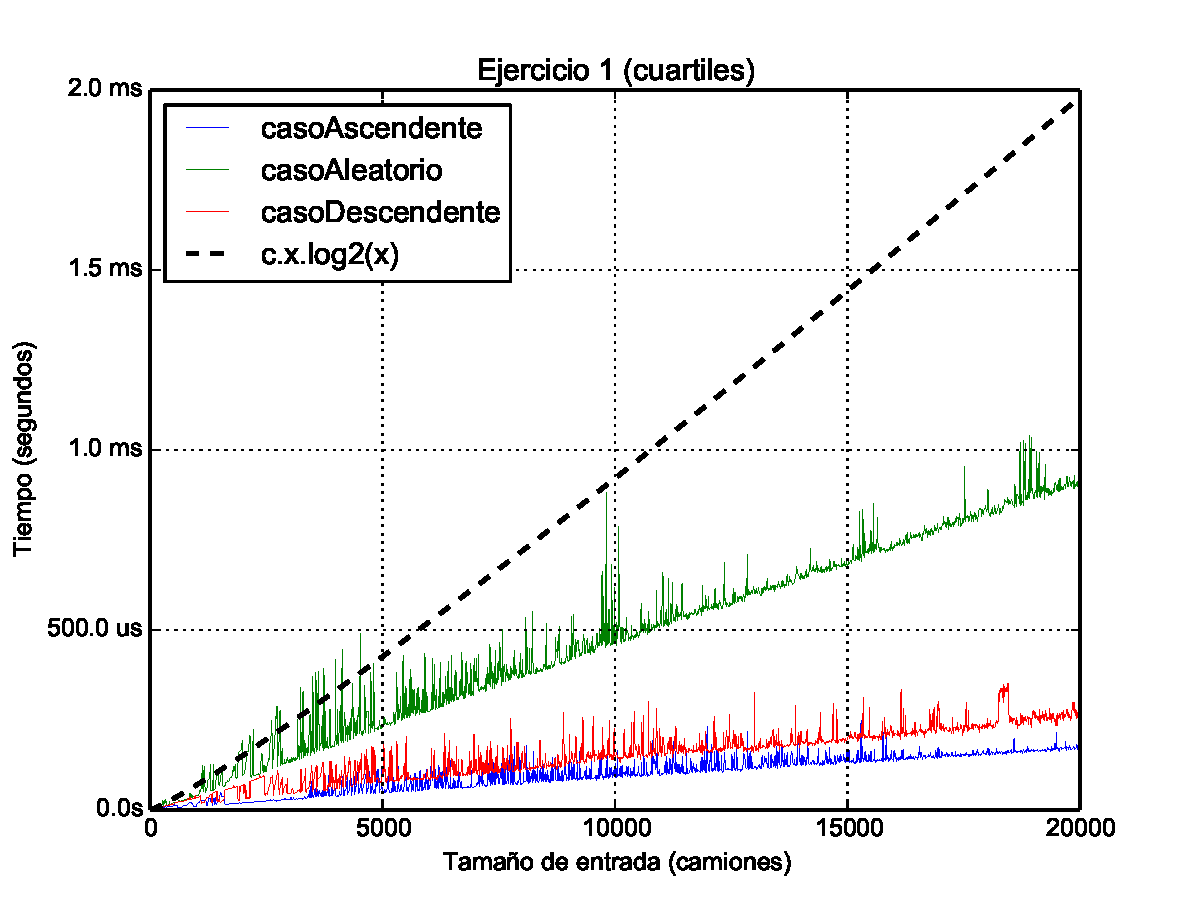
\includegraphics[width=1.4\textwidth,angle=90]{../ej1/graficos/test_1.pdf}
   \caption{\textbf{Muestreo general del Ejercicio 1}}
   \label{fig:ej1-1}
   \end{center}
\end{figure}

\clearpage
\begin{figure}[H]
   \begin{center}
   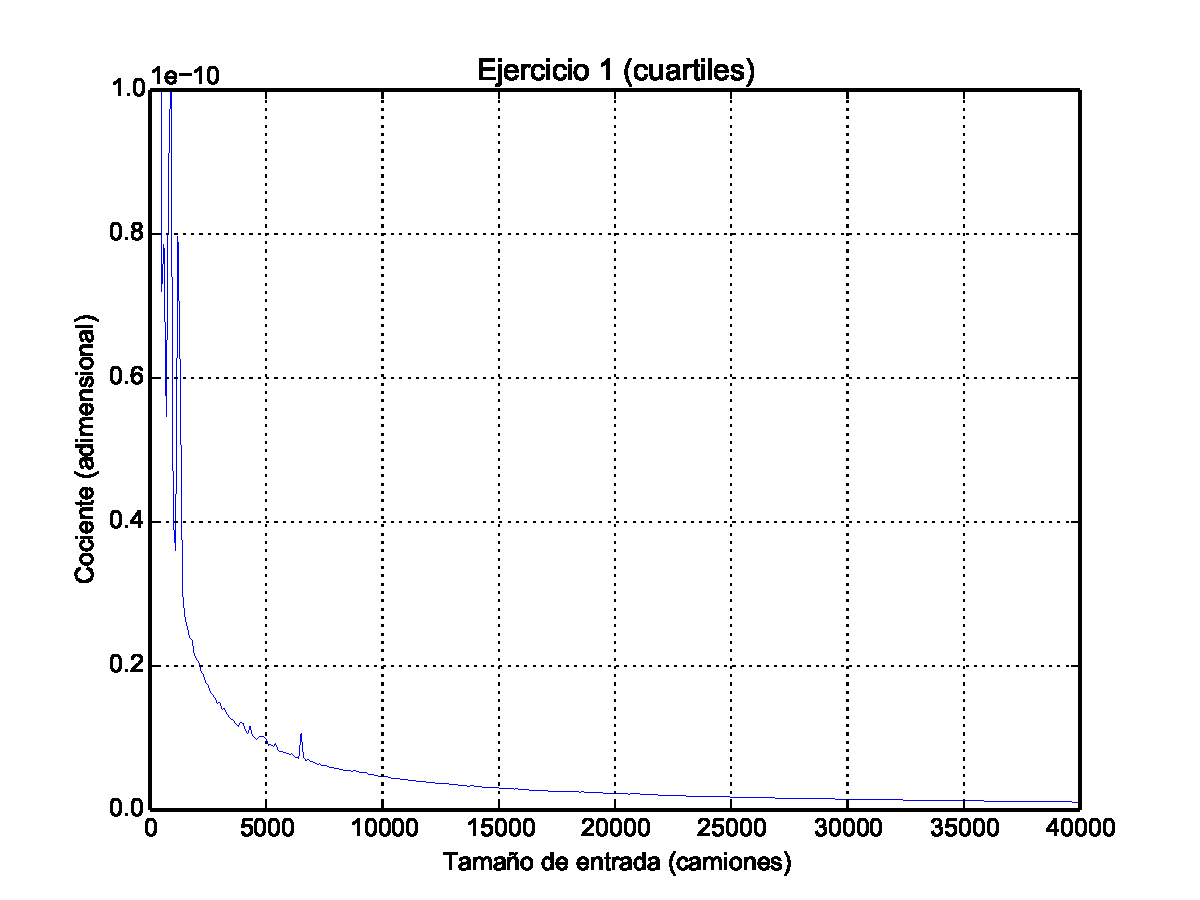
\includegraphics[width=1.4\textwidth,angle=90]{../ej1/graficos/test_2.pdf}
   \caption{\textbf{Relación contra n^{2}}}
   \label{fig:ej1-2}
   \end{center}
\end{figure}

\clearpage
\begin{figure}[H]
   \begin{center}
   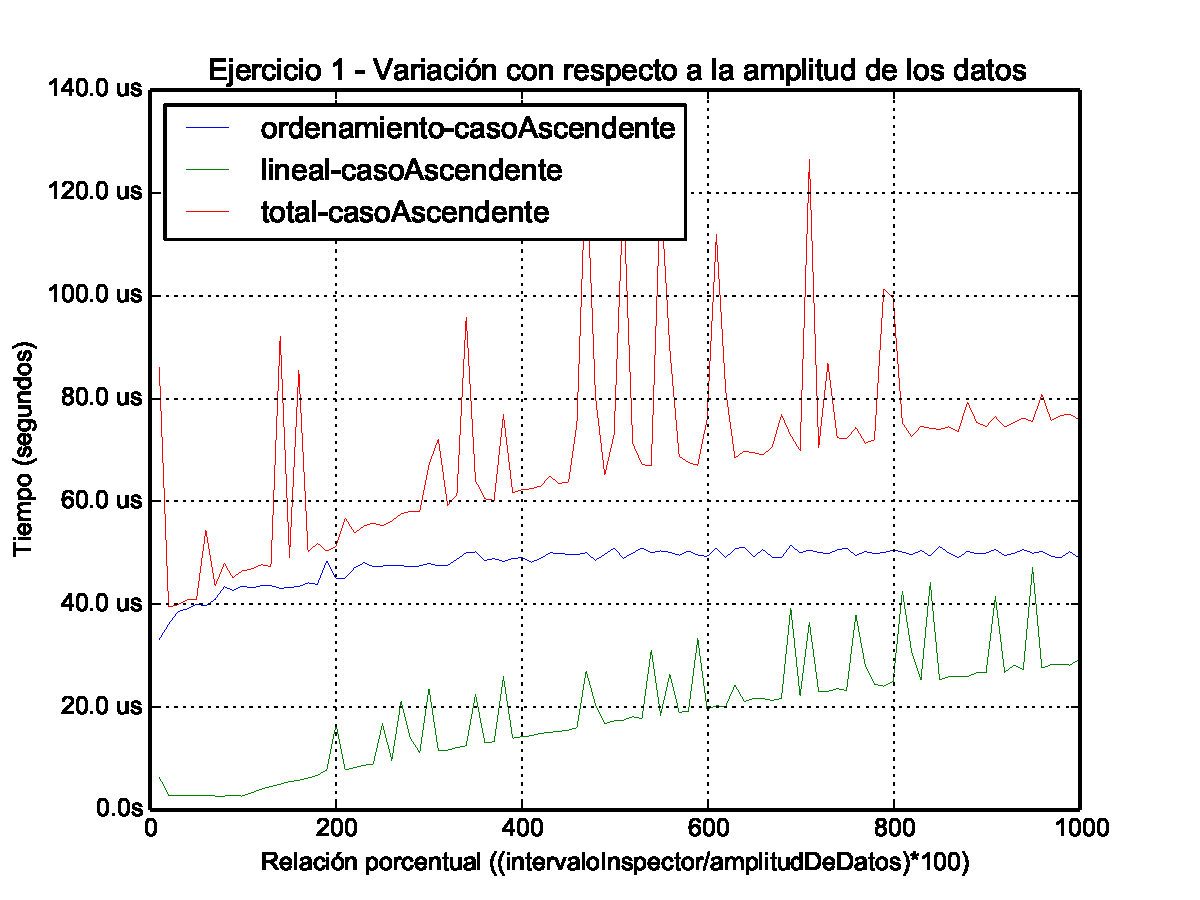
\includegraphics[width=1.4\textwidth,angle=90]{../ej1/graficos/test_3.pdf}
   \caption{}
   \label{fig:ej1-3}
   \end{center}
\end{figure}

%Gráfico1

%Lo siguiente lo dejo escrito pero hay que ver si hay tiempo para hacer todos esos tests... 

%Además, para comprobar que efectivamente la complejidad final está dominada por el algoritmo de sort, se compararon
%los tiempos de la primer parte del algoritmo ($Sort$) y la segunda ($Ciclos$). \\
%Se observa en el siguiente gráfico de $tiempo$ vs $n$:cantidad de camiones, que para el caso del $Sort$ los tiempos
%son mayores, pero siempre por debajo de la complejidad calculada.   

% Gráfico2

%Por último, se compararon los diferentes tiempos según se variaba la longitud $L$ del intervalo formado por 
%la mínima fecha y la máxima fecha en que pasan los camiones, dejando el parámetro $D$ período de contratación del 
%inspector fijo. \\
%Se puede observar que si $D$ es mayor a $L$ el tiempo aumenta como esperábamos, ya que se producen más iteraciones.

% Gráfico3 

% -----------------------------------------------
\end{document}
